%Results
\subsection{Experimental Infrastructure}
Figure~\ref{fig:experimental-setup} shows the infrastructure setup we used to carry out our evaluations.
We used DRAMSim2~\cite{DRAMsim2}, a cycle accurate memory simulation tool, which we customized to incorporate our refresh mechanisms. 
The input traces to DRAMSim2 were generated using the Xilinx Vivado~\cite{vivado} environment in the following manner.
The different accelerators, namely saliency, object recognitoin and action recognition, were implemented in Verilog and their output was used to generate parameters which was fed to a traffic generator.
This traffic generator outputted the memory trace comprising of read and write memory accesses.

\begin{figure}[ht!]
\centering
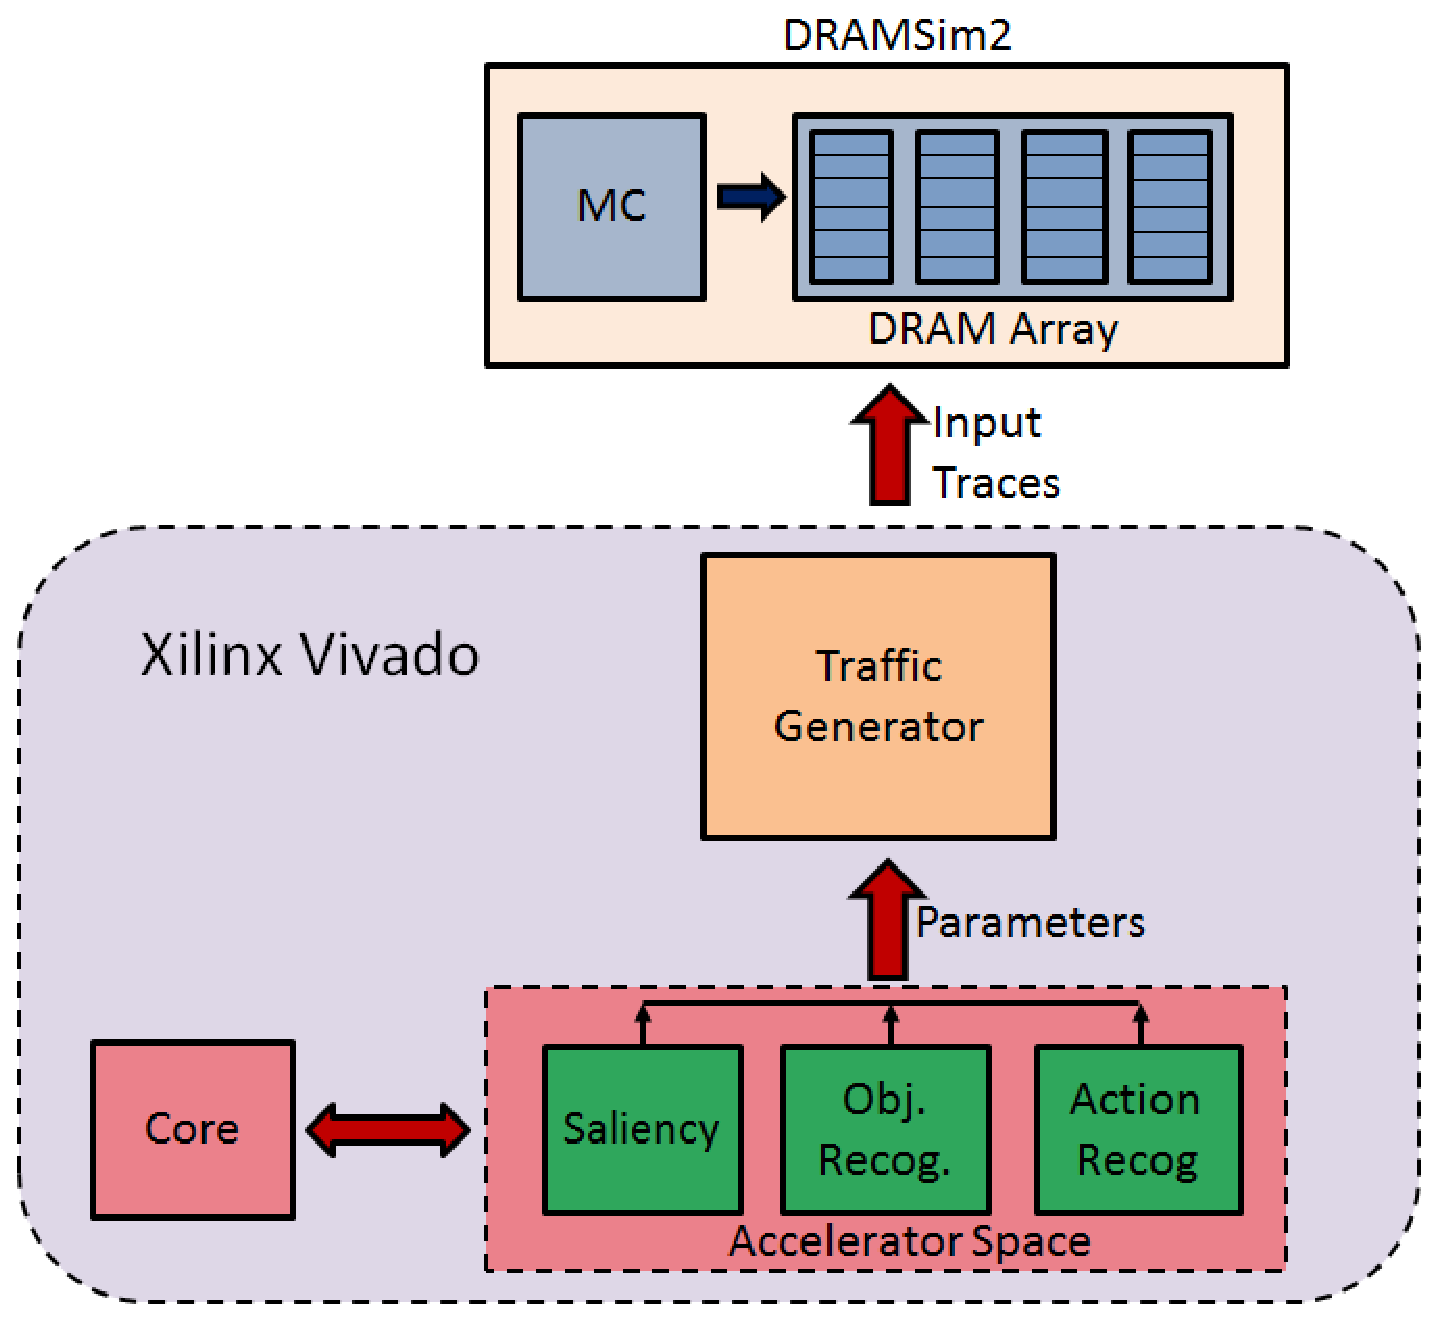
\epsfig{file=figs/experimental_setup.eps, angle=0, width=0.8\linewidth, clip=}
\caption{\label{fig:experimental-setup} Infrastructure setup.}
\end{figure}

\subsection{Sensitivity Analysis}
As shown in Figure~\ref{fig:ActionRecognition}, we evaluated different configurations of action recognition on the Weizmann dataset~\cite{Weizmann}. The results indicate that a purely streaming (no overlap of video segments) configuration affects accuracy considerably (by approximately 10 percent).  

\subsection{Results}
Figure~\ref{fig:PowerResults} illustrates the total power consumption evaluated by feeding the traces generated from Vivado into DRAMSim2. We evaluate our scheme versus our best attempt at modeling Flikker in the given simulator. We also show results when we turn refresh completely off. 

\begin{figure}[ht!]
\centering
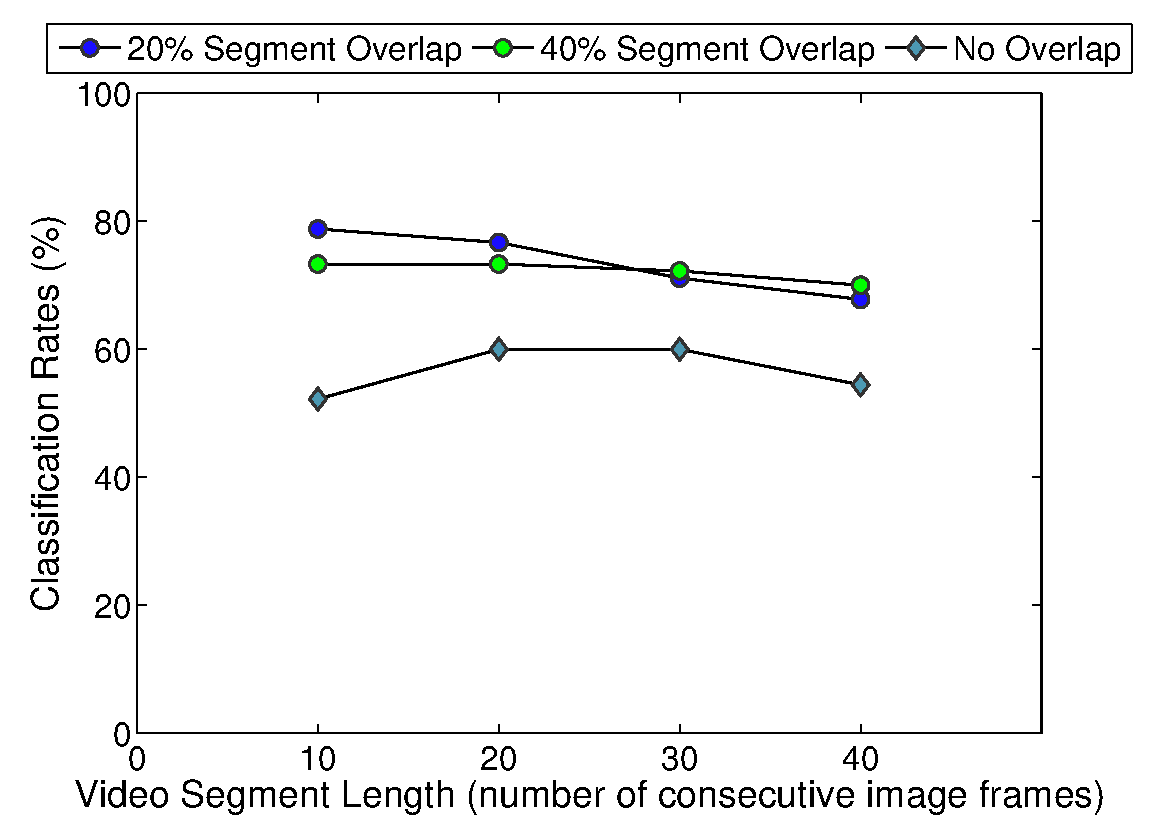
\epsfig{file=figs/ActionRecognitionAnalysis.eps, angle=0, width=0.9\linewidth, clip=}
\caption{\label{fig:ActionRecognition} Accuracy results for different configurations of video segment length and fraction of overlap between segments.}
\end{figure}

\begin{figure}[ht!]
\centering
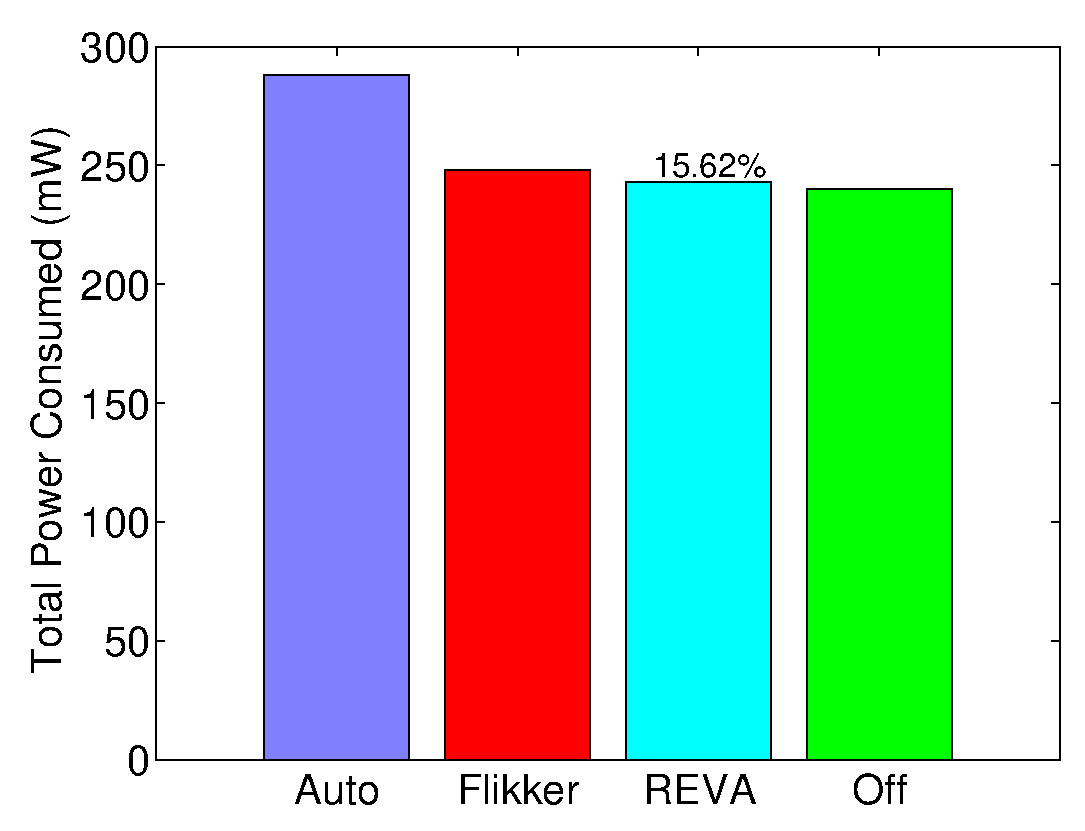
\epsfig{file=figs/DRAMPower_Improvement_8GB.eps, angle=0, width=0.9\linewidth, clip=}
\caption{\label{fig:PowerResults} Power comparisons for different schemes.}
\end{figure}

